\documentclass{article}
\usepackage[T1]{fontenc}
\usepackage{lmodern}
\usepackage{graphicx}
\usepackage{amsmath,amssymb}
\usepackage[a4paper,margin=2cm]{geometry}
\usepackage[absolute,overlay]{textpos}
\setlength{\TPHorizModule}{1mm}
\setlength{\TPVertModule}{1mm}
\usepackage[indonesian]{babel}
\usepackage{hyperref}
\setlength{\emergencystretch}{2em}
% unit: Halaman 11

\begin{document}

% === Halaman 11 (llm) ===

\vspace{150.88mm}

\vspace{80mm}
\begin{center}
\textit{Caesar wheel} untuk membentuk tabel substitusi huruf alfabet
\end{center}

Lihat demo online: \url{https://www.101computing.net/cipher-wheel.html}

% deskripsi: Foto sebuah alat Caesar wheel berwarna emas yang terdiri dari dua lingkaran konsentris dengan huruf alfabet untuk proses enkripsi substitusi.
% bbox normalisasi: [0.2700, 0.2200, 0.6990, 0.7280]
\begin{textblock*}{90.09mm}(56.70mm,65.34mm)
\noindent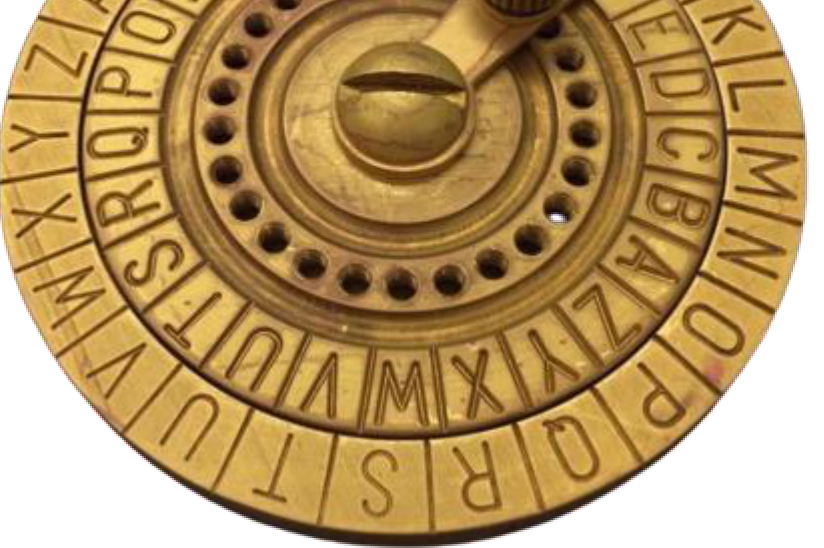
\includegraphics[width=90.09mm,height=150.88mm]{../../images/llm/page_011_img_01.png}%
\end{textblock*}

\end{document}
